\chapter{More Advanced \KK Reduction}

In the previous chapter, it was seen that the \KK reduction of a scalar field on a total spacetime, which is a direct product of a $D$-dimensional spacetime and a compact manifold, is done with ease, but the moral of the procedure is that the effective mass is inversely proportional to the typical length, {\it a.k.a.} radius, of the compact manifold.

Therefore, if there is a phenomenological argument to assume that the compact manifold has a typical radius $R\lll \SI{e-2}{\TeV}$, then only the massless modes of the effective theory are worth tho be analysed. Thus, it is necessary to learn how to count the number of massless fields on the lower dimensional theory. The task is achieved by using topological information of the compact manifold.

\section{Massless Fields and Harmonic Forms}

It was shown in the three examples in Sec.~\ref{sec:KKs:s1}, Sec.~\ref{sec:KKs:s2} and Sec.~\ref{sec:KKs:t2}, when the \KK reduction is done on a compact manifold, $\mathcal{K}$, the massless scalar fields come from the number of nonequivalent harmonic forms on $\mathcal{K}$. This number is independent of the geometry of $\mathcal{K}$, which can be heuristically argued from the fact that is independent or $R$, but is a topological quantity, i.e., a topological invariant.

In a previous chapter, the de Rham cohomology group was defined as
\begin{align}
  H^p(M)\equiv \frac{\Ker\(\df:C^\infty\(\Lambda^{p}(M)\)\to C^\infty\(\Lambda^{p+1}(M)\) \)}{\Im\(\df:C^\infty\(\Lambda^{p-1}(M)\)\to C^\infty\(\Lambda^{p}(M)\)\)},
\end{align}
therefore, the number of nonequivalent harmonic $p$-forms equals the dimension of the $p$-th de Rham cohomology group, which is commonly known as the $p$-th Betti number, $b^p(M)$.

From the previous paragraph, the number of massless scalar fields in the lower dimensional effective theory is $b^0(M)$, while the number of massless 1-forms is $b^1(M)$, and so on! 
Nonetheless, the counting is not necessarily right, since the dimensional reduction of $p$-forms on a compact $n$-dimensional manifold yields to all kind of forms from $(p-n)$ to $p$ order.

In the next sections a heuristic way to compute Betti numbers of simple manifold is shown, and the dimensional reduction of a rich theory is considered.


\section{Cohomology and Homology}

The cohomology groups are not intuitive to calculate. However, de Rham showed that there is a duality between the cohomology group and the homology group.


\begin{Thm}\label{thm:dR}
  If $M$ is a compact manifold, $H^r (M)$ and
  $H_r (M)$ are finite dimensional. Moreover the exists a map
  \begin{align}
    \Lambda    : H^r (M) \times H_r (M) \to \R,
  \end{align}
  which is bilinear and non-degenerate. Thus, $H^ r (M)$ is the dual vector space of $H_r (M)$.
\end{Thm}

From Thm. \ref{thm:dR}, it follows that $b^r(M)=\dim(H^r(M)) = \dim(H_r(M))$, and the later is nothing but the number of nonequivalent, un-shrinkable, $r$-cycles (modulus $r$-boundaries) defined on $M$.  These $r$-cycles can be count via the homotopy group, $\pi_r(M):S^r\to M$.


%% \begin{center}
%%   \begin{tikzpicture}
%%     \begin{axis}[
%%           hide axis,
%%           view={40}{40}
%%       ]
      
%%       \addplot3 [
%%         surf, shader=faceted interp,
%%         point meta=x,
%%         colormap/greenyellow,
%%         samples=20,
%%         samples y=40,
%%         %z buffer=sort,
%%         domain=0:180,
%%         y domain=0:360
%%       ] (
%%                 {sin(x)*cos(y)},
%%                 {sin(x)*sin(y)},
%%                 {cos(x)}
%%       );
      
%%     \end{axis}
%%   \end{tikzpicture}
%% \end{center}

Since the formal theory of this topological invariant is far from the scope of this manuscript, only examples are given in which the $r$-cycles are counted, and finally the {\bf K\"unneth formula} for calculating the Betti numbers of Cartesian products of manifolds is stated.

\subsection{Betti Numbers Though Examples}

Concentrate in the $\pi_0(M)$, for an arbitrary manifold $M$. Since $S^0$ is a point, $b_0(M)$ counts the number of nonequivalent points on $M$, i.e., the number of connected components. Thus,
\begin{align}
  b_0(\R^n)=b_0(S^n)=b_0(T^n) &= 1,\\
  b_0(O(N)) &= 2\qquad\text{for }N>1,
\end{align}
in the last line, $O(N)$ is the $N$-th orthogonal group, and the result is 2 because $O(N)$ has two disconnected components: transformations with $\det(M)=1$ and transformations with $\det(M)=-1$.

One car restate the geometrical meaning of the zeroth Betti number as follows:
\begin{itemize}
\item Imagine a two-dimensional plane.
\item In order to cut it in two parts, one should take out a one-dimensional sub-manifold which can be closed, essentially $S^1$,  or open $\R^1$.
\item This taking out is nothing but a (2-1)-dimensional ``hole'' on $\R^2$. Or in other words, this transformed the connected manifold into two disconnected ones.
\end{itemize}
Therefore, in general the zeroth Betti number counts how many $(D-1)$-dimensional holes  are in a given manifold.

In  the same spirit than before, one can consider $\pi_1(M)$, the set of maps from $S^1\to M$, and count the number of (independent) non-contractible ones. Below,%In Fig. \ref{fig:shrink}, 
the contraction  of a (blue) $S^1$ path to a (red) point is shown.
\begin{center}
  \begin{center}
    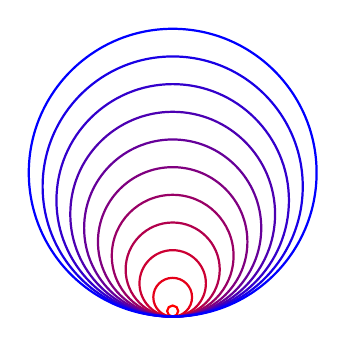
\begin{tikzpicture}[thick]
      \foreach \r in {0,10,...,100}
      \draw[color=blue!\r!red] (0,0) arc  (-90:270:2+.5*\r pt);
    \end{tikzpicture}
  \end{center}
\end{center}

If $M$ is a connected two-dimensional manifold, every circumference should be shrinkable, unless one of the points inside the circumference does not belong to $M$. Therefore,
\begin{align}
  b_0(\R^n)=b_0(S^n)&=0,\\
  b_0\(\R^2-\{0\}\) &= 1.
\end{align}
Moreover, if one ``puncture'' the two-dimensional plane $n$ times, then $b_0\(\R^2-n\{0\}\)=n$.
\begin{center}
  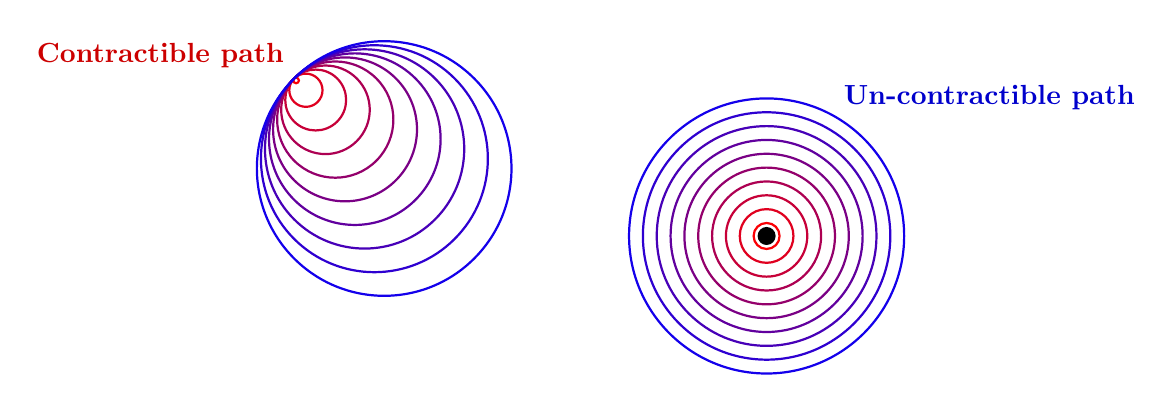
\begin{tikzpicture}[thick]
    \coordinate (P) at (8,2);
    \coordinate (O) at (2,4);
    %\draw[help lines, color=blue!20,step=1cm] (-.4,-.4) grid (12.3,8.3);
    \draw[fill=black] (P) circle (.1cm);
    \foreach \r in {2,12,...,92} {
      \draw[color=blue!\r!red] (O) arc  (-225:135:.5*\r pt);
      \draw[color=blue!\r!red] (P) circle (.5*\r pt+.13cm);}

    \node[anchor=south east] at (O) {\bf{\color{red!80!black}Contractible path}};
    \draw (60:1.7cm) ++(P) node[anchor=south west]   {\bf{\color{blue!80!black} Un-contractible path}};
  \end{tikzpicture}
\end{center}
Once more, a puncture on $\R^2$ is a $(D-2)$-dimensional hole. In fact, the first Betti number counts how many (independent) $(D-2)$-dimensional holes are in a given manifold.

The previous analysis can be carry on and on, and one reach the conclusion that the $n$-th Betti number counts how many independent $(D-n-1)$-dimensional holes are in a $D$-dimensional manifold $M$.



\section{K\"unneth formula}

When a manifold, $M$ is a Cartesian product of other manifolds, say $M_1$ and $M_2$, the topology is determined by the topology of the later. Therefore, their Betti numbers are related. The K\"unneth formula shows that relation,
\begin{align}
  b^n\(M=M_1\times M_2\) = \sum_{p+q=n} b^p\(M_1\)\cdot b^q\(M_2\).\label{KunnethForm}
\end{align}

\begin{WEbox}[frametitle={Betti numbers of a torus ($T^n$)},
  frametitlerule=true,
  frametitlealignment=\centering,
  frametitleaboveskip=10pt,]
  Given the Betti numbers of the 1-sphere, $S^1$,
  \begin{align}
    b^0(S^1) &= 1,\notag\\
    b^1(S^1) &= 1,
  \end{align}
  one can calculate the Betti numbers of $T^n$, since $T^n=\times^n S^1$.

  Using Eq. \eqref{KunnethForm}, it follows that,
  \begin{align}
    b^p(T^n) =\binom{n}{p} = \frac{n!}{p!(n-p)!}.
  \end{align}
\end{WEbox}


\section{Kaluza-Klein spectrum of \M-theory}\

The low energy limit of $\M$-theory is $D=11$ supergravity, when  the spacetime is smooth and large compared with the $11$-dimensional Planck length. So, one can obtain the effective low energy description by consider Kaluza-Klein analysis \cite{Papadopoulos:1995da,Acharya:2004qe}. 

Basically, one will consider the $11$-dimensional background $M^{10,1}$ as a reducible manifolds, $$M^{10,1}=M^{3,1}\times K,$$where $M^{3,1}$ is a maximally symmetric spacetime and $K$ is a compact $7$-dimensional manifold with holonomy group $G_2$.

The only bosonic fields in $D=11$ supergravity are the metric $g$ and the $3$-form $C$. 

\subsection{Expansion of the $C$-form}\

It is  considered that all vacuum expectation value for  the fields vanish, except the one of the metric. Then, considering fluctuations around the vacuum solution, it follows that
\beq
C(x,y)=\delta C(x,y).
\eeq
Therefore, the equation of motion for $C$, 
\begin{align}
  \dfd\;G+\frac{1}{2}G\w G=0,\label{eq:C}
\end{align}
where $G=\df\;C$, can be written to first order in $\delta C$ as
\beq
\dfd \;G=0.
\eeq
As in Maxwell theory, one should impose the gauge condition $\dfd\;C=0$. Since $\La=\acomm{\df\;}{\dfd\;}$, finally the equation of motion is
\beq
\La[11] C=0.
\eeq

Now, splitting $\La[11]=\La[4]+\La[7]$, one notes that for the effective four-dimensional theory, the eigenvalues of $\La[7]$ are like  mass term. Therefore, one proceeds  expanding $C$ in term of the eigen-forms of $K$.

One of the  assumptions of Kaluza-Klein approach is that %as one wants to consider extra dimensions with small radii
the radii of the extra dimensions is small. Then, the only interesting modes in the low energy four-dimensional theory are  massless states. This is because after compactifying the effective four-dimensional mass depends on radii as $m\sim \frac{1}{R}$, so if $R$ is ``really'' small, roughly speaking if it is of Planck length scale, which is $M_{\text{P}}\sim\SI{e-33}{\cm}$, the massive states are too heavy and they will not be considered in the low energy limit.

This allows  to consider the relevant expansion of $C$ just in terms of the harmonic forms on $K$, as 
\beq
C=\phi_I(x)\omega^I(y)+A_\alpha(x)\w\beta^\alpha(y)+\text{ (massive terms)},
\eeq
where $\omega^I$ are basis of the harmonic $3$-forms on $K$, and $\beta^\alpha$ are basis of the harmonic $2$-forms on $K$, so $I=1,...,b_3(K)$ and $\alpha=1,...,b_2(K)$, $x$ are coordinates along $M^4$ and $y$ are coordinates along $K$. Since $C$ is odd under parity, $\phi_I$ describe $b_3(K)$ pseudo-scalars. On the other hand, $A_\alpha$ are  1-forms in Minkowski space, so, they are Abelian gauge fields in four-dimensions.
